%\documentstyle[epsf,twocolumn]{jarticle}       %LaTeX2.09仕様
\documentclass[twocolumn]{jarticle}     %pLaTeX2e仕様

%\usepackage[backend=bibtex, style=numeric]{biblatex}
%\addbibresource{sankou.bib}
%%%%%%%%%%%%%%%%%%%%%%%%%%%%%%%%%%%%%%%%%%%%%%%%%%%%%%%%%%%%%%
%%
%%  基本 バージョン
%%
%%%%%%%%%%%%%%%%%%%%%%%%%%%%%%%%%%%%%%%%%%%%%%%%%%%%%%%%%%%%%%%%
\setlength{\topmargin}{-45pt}
%\setlength{\oddsidemargin}{0cm}
\setlength{\oddsidemargin}{-7.5mm}
%\setlength{\evensidemargin}{0cm}
\setlength{\textheight}{24.1cm}
%setlength{\textheight}{25cm}
\setlength{\textwidth}{17.4cm}
%\setlength{\textwidth}{172mm}
\setlength{\columnsep}{11mm}

\setlength{\intextsep}{8pt}
\setlength{\textfloatsep}{8pt}
\setlength{\floatsep}{1pt}

\kanjiskip=.07zw plus.5pt minus.5pt


%【節がかわるごとに(1.1)(1.2) …(2.1)(2.2)と数式番号をつけるとき】
%\makeatletter
%\renewcommand{\theequation}{%
%\thesection.\arabic{equation}} %\@addtoreset{equation}{section}
%\makeatother

%\renewcommand{\arraystretch}{0.95} 行間の設定

\usepackage[dvipdfmx]{graphicx}   %pLaTeX2e仕様(\documentstyle ->\documentclass)
\usepackage{scalefnt}
\usepackage{bm}
\usepackage{url}
\usepackage{amsmath}
\usepackage{amsfonts}
\usepackage[subrefformat=parens]{subcaption}
\captionsetup{compatibility=false}
%%%%%%%%%%%%%%%%%%%%%%%%%%%%%%%%%%%%%%%%%%%%%%%%%%%%%%%%
\usepackage{comment}
\usepackage{subcaption}
\usepackage{booktabs}
\usepackage{multirow}
\usepackage{nidanfloat}

\begin{document}

\twocolumn[
\noindent
\hspace{1em}

令和2年1月28日(火) 情報工学実験I\hspace{-.1em}I 発表資料
\hfill
\ \ B3 高山 裕成

\vspace{2mm}
\hrule
\begin{center}
{\Large  自然言語処理と深層学習に基づいた 4 コマ漫画のセリフの感情推定}
\end{center}
\hrule
\vspace{3mm}
]

% \footnotesize
\section{はじめに}
近年, 人工知能の基盤である深層学習を始めとする機械学習技術が大きく発展してきている.また, その発展を受けて人工知能を用いた創作物理解が注目されているが, 創作は高次の知的活動であるため, 未だに難しいタスクである.
人の創作物の理解に関する分野の中でもコミック工学など漫画を対象とした研究は, 絵と文章から構成される漫画を対象とするため, 自然言語処理と画像処理の両方の側面を持つマルチモーダルなデータを扱う分野である.コミック工学の分野では様々な研究が報告されているが, その多くは画像処理に基づいた研究であり, 自然言語処理による内容理解を目指した研究は少ない.その一因はデータにある. 漫画に含まれるテキストには, 口語表現, 擬音語, 表記揺れといった漫画特有の言語表現を含み, これらを考慮する必要がある. そして, 漫画が著作物であることに起因する研究用データの不足も課題となっている.

本実験では人工知能を用いた漫画の内容理解の準備として自然言語処理を用いたセリフの感情を推定をする.

\section{研究用コミックデータ}
4 コマ漫画を対象としたデータセットとしては Manga 109 が知られているが, 漫画に登場するキャラクタの感情は明示されていない. そのために人手によるアノテートでラベルを付与する必要があるが, アノテートされたラベルが漫画家の意図とは異なる恐れがある.そこで, 本実験では上野に
よって作られたデータセット\cite{ueno_miki2018} (以下, 4 コマストーリーデータセットとする)を用いる. この 4 コマストーリーデータセットは同一プロットの下, 幾人かの漫画家によって描き下ろされた 4 コマ漫画で構成されており, 作者によって感情ラベルがアノテートされている.
また, 上野は異なる作者によって描かれた 4 コマ漫画を, そのタッチを基に
ギャグタッチ, 少女漫画タッチ, 少年漫画タッチ, 青年漫画タッチ, 萌えタッチと分類している. 図\ref{fig:4koma}にこのデータセットにおける 2 つのタッチのコマ画像の例を示す. 図\ref{fig:4koma}より, 同一プロットであっても, 作者の感性によってアノテートされたラベルが異なっていることが分かる.

\begin{figure}[t]
  \centering
  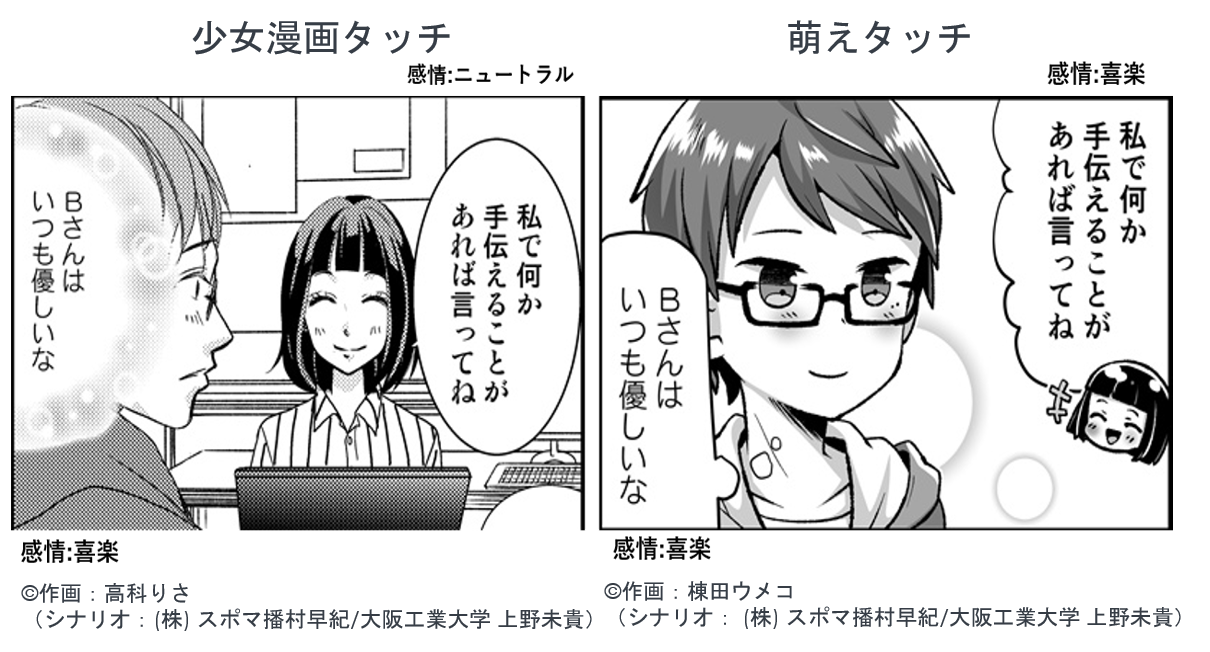
\includegraphics[width=\linewidth]{4koma.png}
  \caption{タッチごとのアノテート例}
  \label{fig:4koma}
\end{figure}

\section{要素技術}
\subsection{Word2Vec, Doc2Vec}
Word2Vec \cite{word2vec} は単語をベクトル空間上に写像して分散表現を得る自然言語処理における重要な手法である.
Word2Vec によって写像したベクトルは, one-hot-vector のような局所表現と異なり, 単語間の意味を考慮した類似度測定や, $「王様」-「男」+「女」=「女王」$のような単語間の意味における演算などができるようになる.
Word2Vec では, 自己から周りの単語あるいは周りの単語から自己を予測することにより分散表現を獲得する.
前者の手法を Skip-gram といい, 後者の手法を Countinuous Bag-of-Words (CBOW)という.

Doc2Vec \cite{word2vec}は文書を分散表現に変換するために Word2Vec に Paragraph ID を導入した拡張手法である.
Paragraph ID は各文書と紐づいており, 単語の学習時に一緒にこの Paragraph ID を学習することで文書の分散表現を獲得する.
CBOW を拡張したモデルを Distributed Memory モデルといい, Skip-gram を拡張したモデルを Distributed Bag-of-Words という. 本実験では, Distributed Memory を用いる.

\subsection{Long Short Term Memory(LSTM)}
LSTM は, 時系列性を有するデータを学習できる Recurrent Neural Network (RNN) の一種である.
RNN は, 前回の出力を現在の入力に追加して再帰的に入力するものであり, 時間方向に展開すると静的なニューラルネットワークとみることができる. RNN の問題点としては, 系列が長くなるにつれて何度も重みが掛けられる回数が多くなり, 勾配が消失(または, 爆発)してしまうことが挙げられる. これに対して, LSTM では重みを掛けずに線形和として過去のデータを保持するため, 長期依存を学習できなくなる問題を解消している.

\section{実験設定}
\subsection{Embedding}
本実験では, Doc2Vec のモデルとして Wikipedia, 小説家になろう, 青空文庫のテキストデータを用いて事前学習させたものを使用する.
このモデルを用いて, JUMAN++ \footnote{http://nlp.ist.i.kyoto-u.ac.jp/index.php?JUMAN++}によって分かち書きされたセリフをそれぞれ 300 次元の分散表現に変換する.

\subsection{Data Augmentation}
4 コマストーリーデータセットの欠点として, データ数が少ないことがあげられる. そこで, 本実験では日本語 WordNet \cite{word_net_jp}のシソーラスを用いてデータを拡張する手法を用いる.
分かち書きされたオリジナルのセリフに対して, 日本語 WordNet で類似語を持つ単語を類似語に置き換えた. ただし, 文の中に類義語を持つ単語が
複数あった場合, 類似語に置き換える単語は同時に 1 つまでとし, 英数字・記号のみで表されている類似語は除外した. 例えば, 5 つの単語からなる文章があり,
各単語が 5 つの類似語を持っている場合, その文からは新しく 25 文が生成されることとなる.

\subsection{実験手法}
本実験では, 各タッチについて感情推定を行った.
本実験で使用するデータセットは全 7 種類の感情ラベル(ニュートラル, 驚愕, 喜楽, 恐怖, 悲哀, 憤怒, 嫌悪)
を持っているが, データ数と解析の難しさの問題から, 今回は喜楽のみを正例, その他を負例とする 2 クラスに分類した.

訓練用データは各タッチの前半 1 話から 5 話までの拡張されたセリフを用い,
評価用データは後半 6 話から 10 話におけるオリジナルのセリフのみを用いた.
表\ref{table:data_size}に各実験で用いたデータ数を示す.
また, 本実験では深層学習のフレームワークとして PyTorch を用いた.

\begin{table}[t]
\centering
\caption{データ数}
\label{table:data_size}
\scalebox{0.7}{
\begin{tabular}{|c|l||c|c|c|c|c|}
\hline
\multicolumn{1}{|l|}{\textbf{}}                      & \textbf{ラベル} & \multicolumn{1}{l|}{\textbf{ギャグ}} & \multicolumn{1}{l|}{\textbf{少女}} & \multicolumn{1}{l|}{\textbf{少年}} & \multicolumn{1}{l|}{\textbf{青年}} & \multicolumn{1}{l|}{\textbf{萌え}} \\ \hline
\multirow{4}{*}{\textbf{train\&valid}}                 & 喜楽        & 15                                & 39                               & 15                               & 18                               & 25                                \\ \cline{2-7}
                                                     & その他       & 40                                & 26                               & 45                               & 44                               & 35                                \\ \cline{2-7}
                                                     & 喜楽(拡張後)   & 1115                              & 2575                             & 940                              & 998                              & 1766                              \\ \cline{2-7}
                                                     & その他(拡張後)  & 2851                              & 1391                             & 3076                             & 3145                             & 2323                              \\ \hline
\multicolumn{1}{|l|}{\multirow{2}{*}{\textbf{test}}} & 喜楽        & 10                                & 38                               & 12                               & 14                               & 22                                \\ \cline{2-7}
\multicolumn{1}{|l|}{}                               & その他       & 56                                & 29                               & 52                               & 51                               & 42                                \\ \hline
\end{tabular}
}
\end{table}

\subsubsection{\small{実験 1 : 時系列を考慮しないセリフの感情推定}}
%ex_main18
識別器として, 3 層からなる多層パーセプトロン (MLP), SVM, RandomForest (RF) を用いた感情推定をして, 各タッチ・手法の結果について比較した. この実験では 1 つのセリフの分散表現を入力することで 1 つの感情ラベルを出力する.
表\ref{table:net_para}に MLP で用いたパラメータ, そして表\ref{table:ex_para}に学習で用いたパラメータを示す. よって, 入力データの次元数はバッチサイズ $\times$ 300 となる.
訓練用データの内 20 \% をサンプリングして検証用データとし,
隠れ層における DropOut 率は 0.5 とした. 出力層でのみ活性化関数として softmax 関数を用いた. また多くのタッチにおいて, 正例は負例に対してデータ数が非常に少ない不均衡データであることから, 損失関数に使うクラス重みとして各タッチについて, 訓練用データの各ラベルのデータ数の逆数を用いた. MLP での識別では検証用データにおける正例の F 値が最大となる epoch のものを評価用モデルとして採用し, SVM と RF での識別では, grid search で得た最良のパラメータを採用した.


\begin{table}
\caption{ネットワークパラメータ}
\label{table:net_para}
\centering
\begin{tabular}{|c||c|c|}
\hline
& MLP & LSTM \\ \hline
(in,hidden,out) & (300,30,2) & (300,300,-)\\ \hline
activation function & tanh & -\\ \hline
\end{tabular}
\end{table}

\begin{table}
\caption{学習パラメータ}
\label{table:ex_para}
\centering
\begin{tabular}{|c||c|c|}
\hline
& \multicolumn{2}{|c|}{実験 $1・2$} \\ \hline
epoch & \multicolumn{2}{|c|}{200}  \\ \hline
batch size & \multicolumn{2}{|c|}{16} \\ \hline
loss function & \multicolumn{2}{|c|}{Cross Entropy Loss} \\ \hline
optimizer & \multicolumn{2}{|c|}{Adam} \\ \hline
learning rate & \multicolumn{2}{|c|}{$5 \times 10^{-6}$} \\ \hline
lr scheduler & \multicolumn{2}{|c|}{CosineAnnealingLR} \\ \hline
\end{tabular}
\end{table}


\subsubsection{\small{実験 2 : 時系列を考慮したセリフの感情推定}}
%ex_main17
実験 1 において MLP に入力していたセリフの分散表現を, LSTM に時系列長分の分散表現を通して得た最後の隠れ層の出力に置き換えることで,
時系列性を考慮した分散表現へと変換されるという推論の下, 時系列長 N が 2 から 6 の場合について, 連続したセリフ N 個を入力し, 末尾のセリフに対応する 1 つの感情ラベルを出力する実験を行い, 各タッチ・時系列長の結果について比較した. MLP のパラメータは実験 1 と同じものを用いた. 表\ref{table:net_para}に LSTM で用いたパラメータ, そして表\ref{table:ex_para}に学習で用いたパラメータを示す. よって, 入力データの次元数は, バッチサイズ $\times$ 時系列長 $\rm N$ $\times$ 300 の 3 次元テンソルとなる. この 4 コマストーリーデータセットは 1 話につき, 2 つの 4 コマを含んでいるが, 各 4 コマは時系列的に繋がっていない. よってセリフの入力列$\{S_i\}$は, 同一の 4 コマに属し, かつ連続しているものを扱う. 各 4 コマの序盤に現れるセリフには過去のセリフが無いため, その分散表現をゼロベクトルとする$``<$pad$>"$を置いてパディングした. また, 入力列の末尾以外のセリフはオリジナルのセリフのみを用い, すべての組み合わせを入力列とすることで, 実験 1 のデータ数と合わせた. 学習時には同様に訓練用データの内 20 \% をサンプリングして検証用データとし, クラス重みも同じものを使った. そして, 検証用データにおける正例の F 値が最大となる epoch のものを評価用モデルとして採用した.

% \begin{figure}[t]
%   \centering
%   \includegraphics[width=\linewidth]{lstm_black.png}
%   \caption{LSTM入力例}
%   \label{fig:lstm}
% \end{figure}


\section{実験結果}
実験 1, 2 において, すべての予測値が負例である場合の各評価指標の値をベースラインとして設定した. 以下, 図における Recall, F 値は正例のものを表し, Acc は全体の精度を表す. また, Recall が 0 の時の F 値は 0 とした.

\subsection{実験 1 : 結果}
表\ref{table:result_1}は各タッチについて, 評価用データの結果をまとめたものである.
表\ref{table:result_1}より, Accにおいてはベースラインを切ったが, Recall, F 値においてはベースラインを超え, 共に MLP において最も高い値を取った. SVM, RF では Recall が 0 だったタッチもあり, 不均衡データにおける分類が上手くいかなかったことが分かった.

\subsection{実験 2 : 結果}
表\ref{table:result_2}は各タッチについて, 評価用データの結果をまとめたものである.
また表\ref{table:result_2}より, 実験 1 と比べるとさらに Acc は落ち込んだが, Recall は全体的に大きく向上しており, F 値にも若干の向上が見られた.
そして時系列長が 6 の時, 5 タッチの平均において Recall, F 値は実験を通して共に最も高い値を取った.


\begin{figure}[tb]
  \centering
  \includegraphics[scale=0.45]{cos_similarity.png}
  \caption{拡張されたセリフのコサイン類似度}
  \label{fig:cos}
\end{figure}

\section{考察}
まず, 各実験の結果についての考察を述べる.
時系列を考慮することで予測が正例に大きく偏ってしまったのは, ネットワークの柔軟性が上がり, クラス重みが強く効きすぎたことで汎化性能が下がったことが原因だと考えられる. そもそも今回の実験で用いたハイパーパラメータは恣意的なものであり, 妥当性を考慮していない. よって optuna などの最適化手法を用いてチューニングをすることで, 各手法において最大性能同士での比較が可能になると考えられる. しかしながら, 実験 2 の結果より感情推定において時系列を考慮することは有用であると分かった.

次に, データの問題点について考察する. まずは Doc2Vec で得た分散表現について, 本実験では Wikipedia や青空文庫のデータをもとに学習したモデルを用いたが, Doc2Vec は前後の文脈よりも登場する単語に強い影響を受けて分散表現を求めるという性質と, 4 コマストーリーデータセットに現れる漫画特有の口語表現や擬音語, 表記揺れはそもそも Doc2Vec のモデルで学習されていない可能性があることから, Manga109 のセリフを併用して追加学習させたり, 他の分散表現化手法についても検討・比較する必要があると考えられる. 次に Data Augmentation の手法について, 図\ref{fig:cos}にギャグタッチにおける拡張されたセリフとそれぞれに対応するオリジナルのセリフとのコサイン類似度を取ったヒストグラムを示す. 図\ref{fig:cos}より, コサイン類似度が 0.5 を下回るデータも少なくなく, このようなものの中にはオリジナルのセリフと大きく意味が異なるものが多かった. また, コサイン類似度に関係なく, 意味は通じるが形容詞であったものが名詞に置き換わっていたり, 文法的に間違ったものも含まれていた. この解決策としては, 形態素の品詞に限定したり, コサイン類似度に閾値を設けることなどが挙げられる. そして, そもそものデータ数が極めて少ないことが問題として挙げられる.

\section{まとめと今後の課題}
本実験では Doc2Vec で得た分散表現から 4 コマストーリーデータセットを用いてセリフの感情推定をした. 時系列を考慮することの有用性を示すことは出来たが, ベースラインを大きく上回る結果とはならなかった.
分散表現化手法や Data Augmentation の手法にはいくつかの改善の余地が見られたため, それらを今後の課題とする. 人間にとっても自然言語のみでの感情推定は難しく, 顔の表情や背景といった画像情報との組み合わせでようやく推定できることが経験則として分かる. このことを踏まえて今後はマルチモーダルな感情推定を試みたい.


% \begin{figure*}[t]
%   \centering
%   \includegraphics[width=\linewidth]{ex1_graph_shounen.png}
%   \caption{実験 1 学習推移 (少年漫画タッチ)}
%   \label{fig:ex1_graph}
% \end{figure*}

\begin{table*}[!b]
\begin{center}
\caption{実験 1 結果(評価用データ)}
\label{table:result_1}
\scalebox{0.75}{
\begin{tabular}{@{}lccccccccccccccc|ccc@{}}
  \toprule
  \multirow{2}{*}{} & \multicolumn{3}{c}{ギャグ} & \multicolumn{3}{c}{少女漫画} & \multicolumn{3}{c}{少年漫画} & \multicolumn{3}{c}{青年漫画} & \multicolumn{3}{c|}{萌え} & \multicolumn{3}{c}{5 タッチ平均} \\
   & Acc & Recall & F 値 & Acc & Recall & F 値 & Acc & Recall & F 値 & Acc & Recall & F 値 & Acc & Recall & F 値 & Acc & Recall & F 値 \\ \midrule
  MLP & 0.77 & 0.10 & 0.12 & 0.51 & 0.55 & 0.56 & 0.73 & 0.08 & 0.11 & 0.62 & 0.50 & 0.36 & 0.66 & 0.36 & 0.42 & 0.66 & \underline{0.32} & \underline{0.31} \\
  SVM & 0.81 & 0.00 &	0.00 & 0.54 & 0.58 & 0.59 & 0.70 & 0.25 & 0.24 & 0.65 & 0.14 & 0.15 & 0.58 & 0.00 & 0.00 & 0.65 & 0.19 & 0.19 \\
  RF & 0.81 & 0.00 & 0.00 & 0.48 & 0.53 & 0.53 & 0.81 & 0.00 & 0.00 & 0.65 & 0.29 & 0.26 & 0.59 & 0.14 & 0.19 & 0.67 & 0.19 & 0.20 \\
 \midrule
  ベースライン & \multicolumn{1}{l}{0.85} & 0.00 & 0.00 & 0.43 & 0.00 & 0.00 & 0.81 & 0.00 & 0.00 & 0.78 & 0.00 & 0.00 & 0.66 & 0.00 & 0.00 & 0.71 & 0.00 & 0.00
\end{tabular}
}
\end{center}
\end{table*}

% \begin{figure*}[t]
%   \centering
%   \includegraphics[width=\linewidth]{ex2_graph_shounen.png}
%   \caption{実験 2 学習推移 (少年漫画タッチ 時系列長 $\rm N = 6$)}
%   \label{fig:ex2_graph}
% \end{figure*}

\begin{table*}[!b]
\begin{center}
\caption{実験 2 結果(評価用データ)}
\label{table:result_2}
\scalebox{0.75}{
\begin{tabular}{@{}lccccccccccccccc|ccc@{}}
  \toprule
\multicolumn{1}{c}{\multirow{2}{*}{時系列長 \rm N}} & \multicolumn{3}{c}{ギャグ} & \multicolumn{3}{c}{少女漫画} & \multicolumn{3}{c}{少年漫画} & \multicolumn{3}{c}{青年漫画} & \multicolumn{3}{c|}{萌え} & \multicolumn{3}{c}{5 タッチ平均} \\
\multicolumn{1}{c}{} & Acc & Recall & F 値 & Acc & Recall & F 値 & Acc & Recall & F 値 & Acc & Recall & F 値 & Acc & Recall & F 値 & Acc & Recall & F 値 \\ \midrule
2 & 0.48 & 0.70 & 0.29 & 0.49 & 0.76 & 0.63 & 0.56 & 0.33 & 0.22 & 0.57 & 0.64 & 0.39 & 0.45 & 0.77 & 0.49 & 0.51 & 0.64 & 0.41 \\
3 & 0.52 & 0.60 & 0.27 & 0.46 & 0.79 & 0.63 & 0.55 & 0.42 & 0.26 & 0.51 & 0.57 & 0.33 & 0.47 & 0.73 & 0.48 & 0.50 & 0.62 & 0.39 \\
4 & 0.59 & 0.60 & 0.31 & 0.52 & 0.87 & 0.67 & 0.47 & 0.33 & 0.19 & 0.45 & 0.71 & 0.36 & 0.45 & 0.73 & 0.48 & 0.50 & 0.65 & 0.40 \\
5 & 0.47 & 0.70 & 0.29 & 0.55 & 0.84 & 0.68 & 0.52 & 0.25 & 0.16 & 0.45 & 0.71 & 0.36 & 0.44 & 0.77 & 0.49 & 0.48 & 0.66 & 0.39 \\
6 & 0.39 & 0.70 & 0.26 & 0.52 & 0.87 & 0.67 & 0.61 & 0.50 & 0.32 & 0.57 & 0.71 & 0.42 & 0.48 & 0.77 & 0.51 & 0.52 & \underline{0.71} & \underline{0.44} \\ \midrule
ベースライン & \multicolumn{1}{l}{0.85} & 0.00 & 0.00 & 0.43 & 0.00 & 0.00 & 0.81 & 0.00 & 0.00 & 0.78 & 0.00 & 0.00 & 0.66 & 0.00 & 0.00 & 0.71 & 0.00 & 0.00
\end{tabular}
}
\end{center}
\end{table*}


\bibliographystyle{unsrt}
\bibliography{sankou}
\end{document}
